\documentclass[conference]{IEEEtran}
\IEEEoverridecommandlockouts
% The preceding line is only needed to identify funding in the first footnote. If that is unneeded, please comment it out.
\usepackage{cite}
\usepackage{amsmath,amssymb,amsfonts}
\usepackage{algorithmic}
\usepackage{graphicx}
\usepackage{textcomp}
\usepackage{xcolor}
\def\BibTeX{{\rm B\kern-.05em{\sc i\kern-.025em b}\kern-.08em
    T\kern-.1667em\lower.7ex\hbox{E}\kern-.125emX}}
\begin{document}

\title{RBE 501 Week 1 Assignment}

\author{\IEEEauthorblockN{1\textsuperscript{st} Arjan Gupta}
\IEEEauthorblockA{\textit{Robotics Engineering} \\
\textit{Worcester Polytechnic Institute}\\
Worcester, MA, USA \\
agupta11@wpi.edu}
}

\maketitle

\begin{abstract}
This document provides an in-depth solution for Problem 2--37 described in
Robot Modeling and Control.
This is the assignment for the first week in RBE 501 (Robot Dynamics),
Spring 2023 at Worcester Polytechnic Institute.
\end{abstract}

\begin{IEEEkeywords}
robotics, homogeneous transformation, frames
\end{IEEEkeywords}

\section{Introduction}
We are asked to solve Problem 2--37 of the main textbook~\cite{Spong2006}. Here,
a robot is near a table, with a camera placed over the table to supervise the
robot. A cube is also placed in the center of the table-top. 
The objective of the problem is to express all the frames in the environment
(frame for the edge of the table, frame for the cube,
and frame for the overhead camera) in terms of the homogeneous transformations with
respect to the base frame, situated at the base link of the robot. An additional
objective of the problem is to find the homogeneous transformation relating
the center of the cube's frame to the camera's frame. The graphic below, given
in the textbook, gives a pictorial representation of the problem.
\begin{figure}[h]
    \centering
    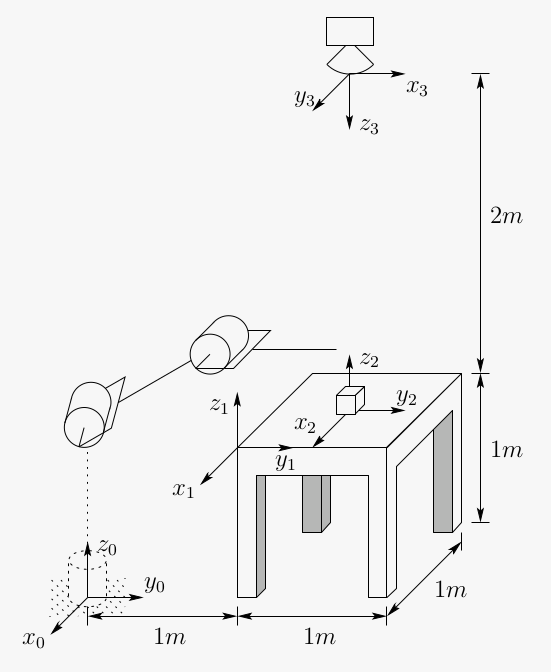
\includegraphics[scale=0.4]{./prob3-37-fig.png}
    \caption{Figure for 2--37}
\end{figure}

\section{Materials and Methods}

We know from the textbook~\cite{Spong2006} that given a rotational matrix $R$, and
a rigid translation $d$, we have the following definition of
a homogeneous transformation,
\[
    H = \begin{bmatrix}
        R & d\\
        0 & 1
    \end{bmatrix}; R \in SO(3), d \in \mathbb{R}^3
\]
Also, the homogeneous transformation $H^m_n$ describes the transformation
of frame $n$ with respect to $m$.
Therefore, given our objectives, and the frames as numbered in Figure 1, 
we need to find $H^0_1$, $H^0_2$, $H^0_3$, and $H^3_2$.

\bibliography{refs.bib}
\bibliographystyle{IEEEtran}

\end{document}